%! TEX root = main.tex

This section presents the verification and validation (V\&V) of our PINN solvers and PetIBM, an in-house CFD solver \cite{chuang_petibm_2018}.
V\&V results are necessary to build confidence in our case study described later in section \ref{sec:case-study}.
For verification, we solved a 2D Taylor-Green vortex (TGV) at Reynolds number $Re=\num{100}$, which has a known analytical solution.
For validation, on the other hand, we use 2D cylinder flow at $Re=40$, which exhibits a well-known steady state solution with plenty of experimental data available in the published literature.

\subsection{Verification: 2D Taylor-Green Vortex (TGV), $Re=\num{100}$}\label{sec:verification}

Two-dimensional Taylor-Green vortices with periodic boundary conditions have closed-form analytical solutions,
and serve as standard verification cases for CFD solvers.
We used the following 2D TGV configuration, wih $Re=\num{100}$, to verify both the PINN solvers and PetIBM:
\begin{equation}\label{eq:tgv}
    \left\{
        \begin{aligned}
            u(x, y, t) &= \cos(x)\sin(y)\exp(-2 \nu t) \\
            v(x, y, t) &= - \sin(x)\cos(y)\exp(-2 \nu t) \\
            p(x, y, t) &= -\frac{\rho}{4}\left(\cos(2x) + \cos(2y)\right)\exp(-4 \nu t)
        \end{aligned}
    \right.
\end{equation}
where $\nu=\num{0.01}$ and $\rho=\num{1}$ are the kinematic viscosity and the density, respectively.
The spatial and temporal domains are $x, y \in \left[-\pi, \pi\right]$ and $t \in [0, 100]$.

Periodic conditions are applied at all boundaries by modifying the inputs of the neural network $G$: $x$ and $y$ are periodic at $-\pi$ and $\pi$, so instead of using $G=G(x, y, t)$, we modified the neural network $G$ to
\begin{equation}\label{eq:periodic-bc}
    G = G(\sin(x), \cos(x), \sin(y), \cos(y), t)
\end{equation}
This approach builds the periodicity into the model directly, and hence no boundary losses are needed.
In general, says, if $x$ is periodic at $x_1$ adn $x_2$, to build the periodicity in to the neural networks, one can change the inputs to neural networks of $\sin({2\pi\frac{x-x_1}{x_2-x_1}})$ and $\cos({2\pi\frac{x-x_1}{x_2-x_1}})$.

In PetIBM, we used the Adams-Bashforth and the Crank-Nicolson schemes for the temporal discretization of convection and diffusion terms, respectively.
The spatial discretization is central difference for all terms.
Theoretically, we expect to see second-order convergence in both time and space for this 2D TGV problem in PetIBM.
We used the following $L_2$ spatial-temporal error to examine the convergence:
\begin{equation}\label{eq:spt-err-def}
    \begin{aligned}
    L_{2,sp-t} \equiv &\sqrt{
        \frac{1}{L_x L_y T}
        \iiint\limits_{x, y, t} \lVert f - f_{ref} \rVert^2 \diff x \diff y \diff t
    } \\
    = &
    \sqrt{\frac{1}{N_x N_y N_t}\sum\limits_{i=1}^{N_x}\sum\limits_{j=1}^{N_y}\sum\limits_{k=1}^{N_t}\left(f^{(i, j, k)} - f_{ref}^{(i, j, k)}\right)^2}
    \end{aligned}
\end{equation}
Here, $N_x$, $N_y$, and $N_t$ represent the number of solution points in $x$, $y$, and $t$;
$L_x$ and $L_y$ are the domain lengths in $x$ and $y$;
$T$ is the total simulation time;
$f$ is the flow quantity of interest, while $f_{ref}$ is the corresponding analytical solution.
The superscript $(i, j, k)$ denotes the value at the $(i, j, k)$ solution point in the discretized spatial-temporal space.
We used Cartesian grids with $2^{n} \times 2^{n}$ cells for $i=4$, $5$, $\dots$, $10$.
The time step size $\Delta t$ does not follow a fixed refinement ratio, and takes the values $\Delta t = \num{1.25e-1}$, $\num{8e-2}$, $\num{4e-2}$, $\num{2e-2}$, $\num{1e-2}$, $\num{5e-3}$, and $\num{1.25e-3}$, respectively.
$\Delta t$ was determined based on the maximum allowed CFL number and whether it was a factor of $2$ to output transient results every $\num{2}$ simulation seconds.
The velocity and pressure linear systems were both solved with BiCGSTAB (bi-conjugate gradient stabilized method).
The preconditioners of the two systems are the block Jacobi preconditioner and the algebraic multigrid preconditioner from NIVIDA's AmgX library.
At each time step, both linear solvers stop when the preconditioned residual reaches \num{e-14}.
The hardware used for PetIBM simulations contains 5 physical cores of Intel E5-2698 v4 and 1 NVIDIA V100 GPU.

Figure \ref{fig:tgv-petibm-convergence} shows the spatial-temporal convergence results of PetIBM.
\begin{figure}
    \centering%
    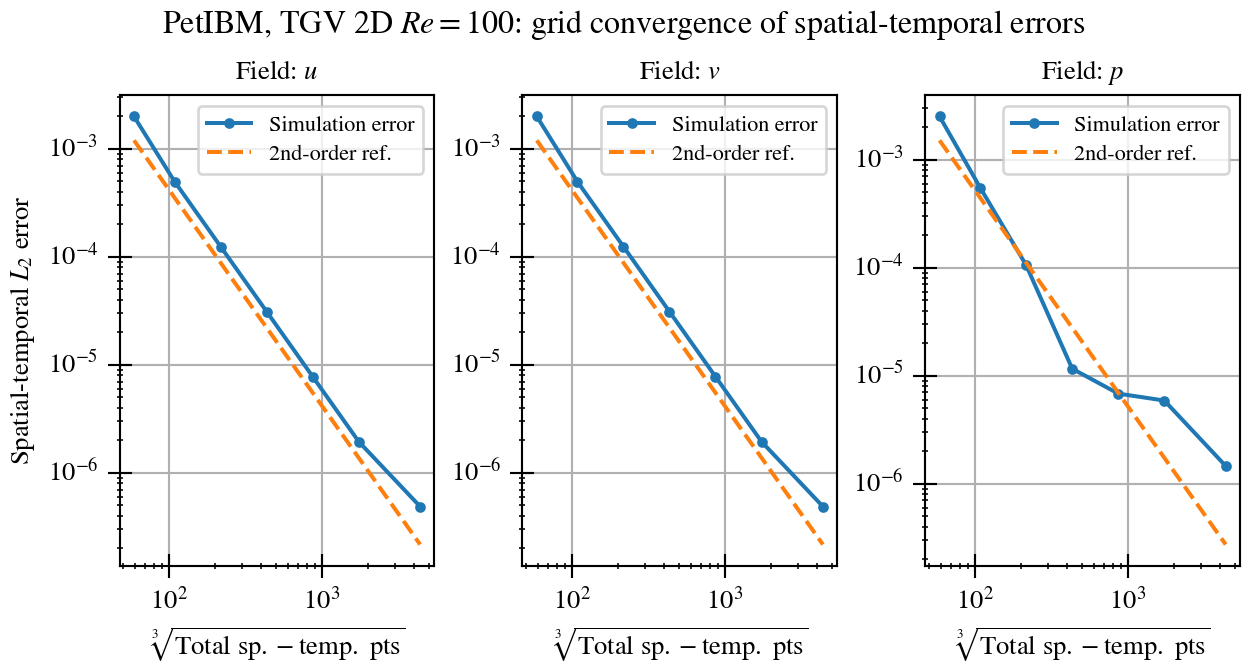
\includegraphics[width=\columnwidth]{tgv-2d-re100/petibm-tgv-2d-re100-convergence}%
    \caption{%
        Grid-convergence test and verification of PetIBM using 2D TGV at $Re=\num{100}$.
        The spatial-temporal $L_2$ error is defined in equation \eqref{eq:spt-err-def}.
        Taking the cubic root of the total spatial-temporal solution points gives the characteristic cell size.
        Both $u$ and $v$ velocities follow second-order convergence, while the pressure $p$ follows the trend with some fluctuation.
    }
    \label{fig:tgv-petibm-convergence}%
\end{figure}
Both $u$ and $v$ follow an expected second-order convergence before the machine round-off errors start to dominate on the $1024 \times 1024$ grid.
The pressure follows the expected convergence rate with some fluctuations.
Further scrutiny revealed that the AmgX library was not solving the pressure system to the desired tolerance.
The AmgX library has a hard-coded stop mechanism when the relative residual (relative to the initial residual) reaches machine precision.
So while we configured the absolute tolerance to be \num{e-14}, the final preconditioned residuals of the pressure systems did not match this value.
On the other hand, the velocity systems were solved to the desired tolerance.
With this minor caveat, we consider the verification of PetIBM to be successful, as the minor issue in the convergence of pressure is irrelevant to the code implementation in PetIBM.

Next, we solved this same TGV problem using an unsteady PINN solver.
For the optimization, we used PyTorch's Adam optimizer
with the following parameters: $\beta_1=\num{0.9}$, $\beta_2=\num{0.999}$, and $\epsilon=\num{e-8}$.
The total iteration number in the optimization is \num{400000}.
Two learning-rate schedulers were tested: the exponential learning rate and the cyclical learning rate.
Both learning rates are from PyTorch and were used merely to satisfy our curiosity.
The exponential scheduler has only one parameter in PyTorch: $\gamma=0.95^{\frac{1}{5000}}$.
The cyclical scheduler has the following parameters: $\eta_{low}=\num{1.5e-5}$, $\eta_{high}=\num{1.5e-3}$, $N_c=\num{5000}$, and $\gamma=\num{9.99989e-1}$.
These values were chosen so that the peak learning rate at each cycle is slightly higher than the exponential rates.
Figure \ref{fig:tgv-learning-rate-hist} shows a comparison of the two schedulers.

\begin{figure}
    \centering%
    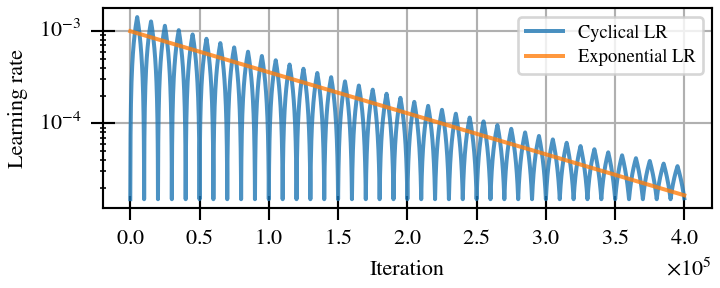
\includegraphics[width=\columnwidth]{tgv-2d-re100/learning-rate-hist}%
    \caption{%
        Learning-rate history of 2D TGV $Re=\num{100}$ w/ PINN
        The exponential learning rate scheduler is denoted as {\it Exponential}, and the cyclical scheduler is denoted as {\it Cyclical}.
    }
    \label{fig:tgv-learning-rate-hist}%
\end{figure}

The MLP network used consisted of \num{3} hidden layers and \num{128} neurons per layer.
\num{8192e4} spatial-temporal points were used to evaluate the PDE losses (i.e., the $L_1$, $L_2$, and $L_3$ in figure \ref{fig:pinn-workflow}).
We randomly sampled these spatial-temporal points from the spatial-temporal domain$\left[-\pi, \pi\right] \times \left[-\pi, \pi\right] \times \left(0, 100\right]$.
During each optimization iteration, however, we only used \num{8192} points to evaluate the PDE losses.
It means the optimizer sees each point \num{40} times on average because we have a total of \num{4e5} iterations.
Similarly, \num{8192e4} spatial-temporal points were sampled from $x,y \in \left[-\pi, \pi\right] ] \times \left[-\pi, \pi\right]$ and $t=0$ for the initial condition loss (i.e., $L_4$ to $L_6$).
And the same number of points were sampled from each domain boundary ($x=\pm\pi$ and $y=\pm\pi$) and $t\in\left(0, 100\right]$ for boundary-condition losses ($L_7$ to $L_{10}$).
A total of \num{8192} points were used in each iteration for these losses as well.

We used one NVIDIA V100 GPU to run the unsteady PINN solver for the TGV problem.
Note that the PINN solver used single-precision floats, which is the default in PyTorch.

After training, we evaluated the PINN solver's errors at cell centers in a $512$ $\times$ $512$ Cartesian grid and at $t=0$, $2$, $4$, $\cdots$, $100$.
Figure \ref{fig:tgv-pinn-loss} shows the histories of the optimization loss and the $L_2$ errors at $t=0$ and $t=40$ of the $u$ velocity on the left vertical axis.
The reader should not confuse these two different metrics: whereas the prediction accuracy (measured by the $L_2$ errors) is the primary concern, the optimization loss is only a proxy for the accuracy.
The optimization loss is a combination of the PDE losses and the initial and boundary condition losses, and it depends on how one optimizes the neural network parameters.
\begin{figure}
    \centering%
    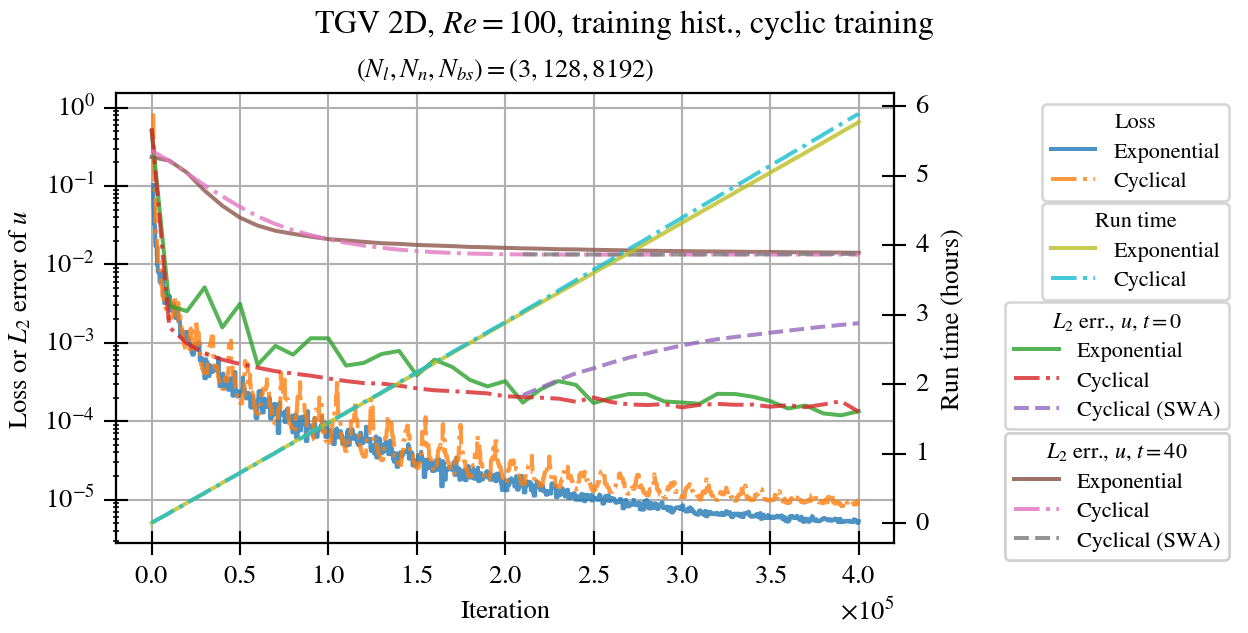
\includegraphics[width=\columnwidth]{tgv-2d-re100/pinn-nl3-nn128-npts8192-convergence}%
    \caption{%
        Histories with respect to optimization iterations for the total loss and the $L_2$ errors of $u$ at $t=0$ and $40$ in the TGV verification of the unsteady PINN solver.
        On the left vertical axis is the magnitude of the total loss and the errors.
        (Note that loss is merely a proxy for the accuracy, whereas the error measures it directly.)
        On the right vertical axis is the run time.
        The cyclical scheduler has a slightly better accuracy at $t=40$ with a slightly more time cost, though its total loss is higher.
    }
    \label{fig:tgv-pinn-loss}%
\end{figure}
The same figure also shows the run time (wall time) on the right vertical axis.
The total loss converges to an order of magnitude of \num{e-6}, which may reflect the fact that PyTorch uses single-precision floats.
The errors at $t=0$ and $t=40$ converge to the orders of \num{e-4} and \num{e-2}, respectively.
This observation is reasonable because the net errors over the whole temporal domain is, by definition, similar to the square root of the total, which is \num{e-3}.
The PINN solver got exact initial conditions for training (i.e., $L_4$ to $L_6$), so it is reasonable to see a better prediction accuracy at $t=0$ than later times.
Finally, though the computational performance is not the focus of this paper, for the interested reader's benefit we would like to point out that the PINN solver took about 6 hours to converge with a V100 GPU, while PetIBM needed less than 10 seconds to get an error level of \num{e-2} using a very dated K40 GPU (and most of the time was overhead to initialize the solver).

In sum, we determined the PINN solution to be verified, although the accuracy and the computational cost were not satisfying.
The relatively low accuracy is likely a consequence of the use of single-precision floats and the intrinsic properties of PINNs, rather than implementation errors.
Figure \ref{fig:tgv-pinn-contours} shows the contours of the PINN solver's predictions at $t=40$ for reference.
For more details about this verification exercise, we refer readers to our conference proceedings paper \cite{chuang_experience_2022}.

\begin{figure}[t]
    \centering%
    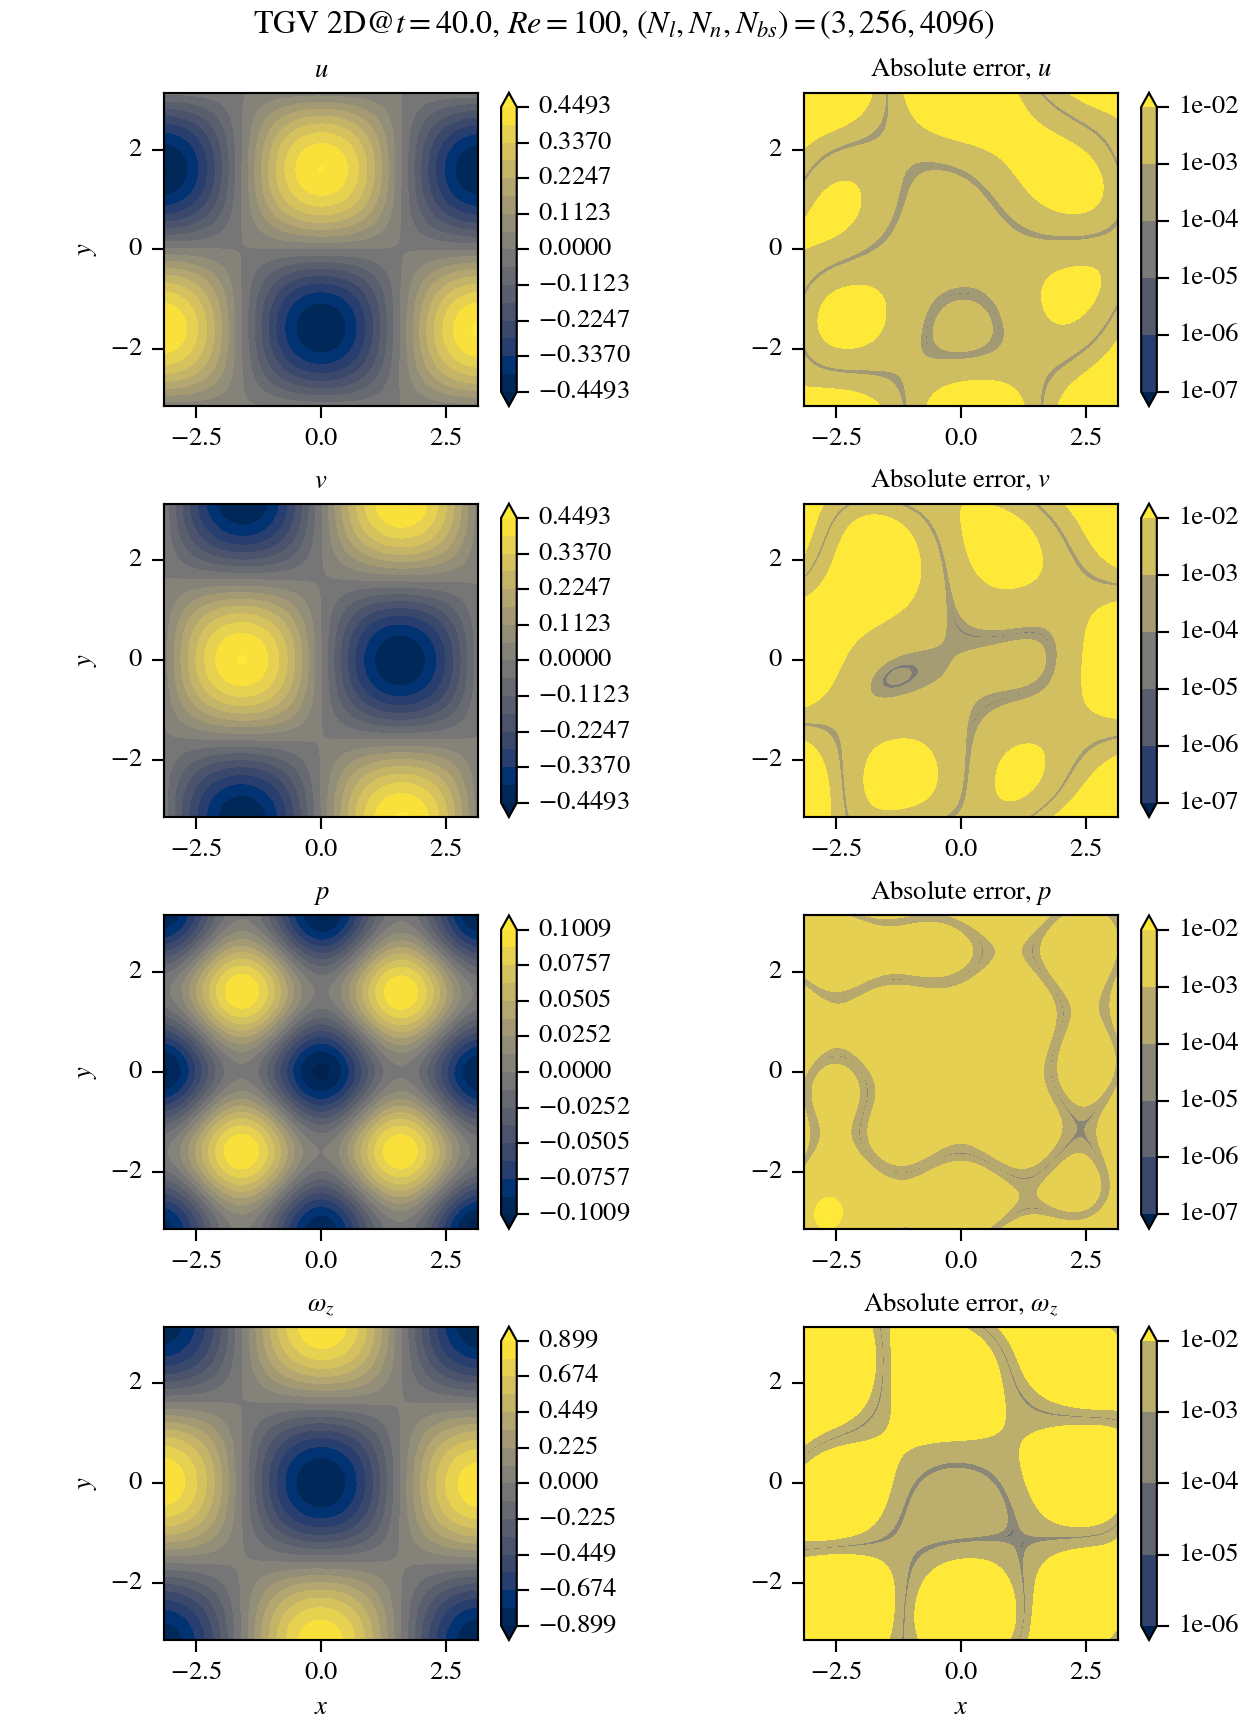
\includegraphics[width=0.95\columnwidth]{tgv-2d-re100/pinn-nl3-nn256-npts4096-contours.png}
    \caption{%
        Contours at $t=40$ of 2D TGV at $Re=\num{100}$ primitive variables and errors using the unsteady PINN solver.
        Roughly speaking, the absolute errors are at the level of \num{e-3} for primitive variables ($u$, $v$, and $p$), which corresponds to the square root of the total loss.
        The vorticity was obtained from post-processing and hence was augmented in terms of errors.
    }
    \label{fig:tgv-pinn-contours}%
\end{figure}

% vim:ft=tex: